\documentclass[a4paper]{scrartcl}
\usepackage[english]{babel}
\usepackage[top=2cm,bottom=3cm,left=2.5cm,right=2.5cm]{geometry}
\usepackage[colorlinks=true, allcolors=black]{hyperref}
\usepackage{wrapfig} %문단 내 이미지 삽입
\usepackage{graphicx} %색상
\usepackage{overpic}
\usepackage[normalem]{ulem}%취소선
\usepackage{array} %표
\usepackage{mdframed, tcolorbox} %글상자
\usepackage[yyyymmdd]{datetime}
	\renewcommand{\dateseparator}{--}
\usepackage{amsmath, amsfonts, amssymb, bm} %수식
	\DeclareMathOperator{\arccsc}{arccsc}
	\DeclareMathOperator{\arcsec}{arcsec}
	\DeclareMathOperator{\arccot}{arccot}
	\DeclareMathOperator{\csch}{csch}
	\DeclareMathOperator{\sech}{sech}
	\DeclareMathOperator{\arcsinh}{arcsinh}
	\DeclareMathOperator{\arccosh}{arccosh}
	\DeclareMathOperator{\arctanh}{arctanh}
	\DeclareMathOperator{\arccsch}{arccsch}
	\DeclareMathOperator{\arcsech}{arcsech}
	\DeclareMathOperator{\arccoth}{arccoth}
	
	\DeclareMathOperator{\meter}{m}
	\DeclareMathOperator{\cm}{cm}
	\DeclareMathOperator{\mm}{mm}
	\DeclareMathOperator{\mum}{\mu m}
	\DeclareMathOperator{\newton}{N}
	\DeclareMathOperator{\kn}{kN}
	\DeclareMathOperator{\kgf}{kgf}
	\DeclareMathOperator{\pa}{Pa}
	\DeclareMathOperator{\kpa}{kPa}
	\DeclareMathOperator{\mpa}{MPa}
	\DeclareMathOperator{\gpa}{GPa}
	\DeclareMathOperator{\npm}{N/m}
	\DeclareMathOperator{\knpm}{kN/m}
	\DeclareMathOperator{\kph}{km/h}
	\DeclareMathOperator{\mps}{m/s}
	\DeclareMathOperator{\tkph}{kph}
	\DeclareMathOperator{\tmps}{mps}
	\DeclareMathOperator{\mpss}{m/s^2}
	\DeclareMathOperator{\dgr}{\!^\circ}
	\DeclareMathOperator{\cel}{\!^\circ C}
	\DeclareMathOperator{\kg}{kg}
	\DeclareMathOperator{\kgpcm}{kg/m^3}
	\DeclareMathOperator{\nm}{N\cdot m}
	\DeclareMathOperator{\knm}{kN\cdot m}
	\DeclareMathOperator{\kw}{kW}
	\DeclareMathOperator{\kwh}{kWh}
	\DeclareMathOperator{\mmhg}{mmHg}
	\DeclareMathOperator{\snd}{s}
\usepackage{polynom} %나눗셈 필산
\usepackage{cancel} %수식 약분선
\usepackage{titlesec} %섹션 이름 변경
	\titlespacing*{\section}{3mm}{0mm}{1mm}
	\titleformat{\section}{\bfseries\large}{}{0ex}{}
\usepackage{kotex} %한글

\newcommand{\prob}[2]{\section{#1}\begin{mdframed}#2\end{mdframed}}

\newlength{\picwidth}
\newcommand{\probpic}[4]{
	\setlength{\picwidth}{145mm}\addtolength{\picwidth}{-#3}\section{#1}\begin{mdframed}\begin{tabular}{m{#3}m{\picwidth}}
	\includegraphics[width = #3]{#2} & #4\end{tabular}\end{mdframed}
	}

\title{\vspace{100pt}\Huge{HW2}}
\author{
	2025-2 구조역학(박성훈 교수님)\\[10pt]
	Problem 7.132, 7.135, 8.4, 8.13, 문제1, 문제2\\[100pt]
	오류 제보\quad eusnoohong03@soongsil.ac.kr\\
	}
\date{\today}

\begin{document}
	
\renewcommand*{\titlepagestyle}{empty}
\maketitle

\vspace{60pt}

\begin{center}
	\includegraphics[width=0.45\textwidth]{SSU symbol KR-EN.jpg}
\end{center}

\newpage\setcounter{page}{1}

\setlength{\parindent}{0pt}

\prob{Problem 7.132}{For the given state of plane strain, use Mohr's circle to determine the state of plane strain associated with axes $x'$ and $y'$ rotated through the given angle $\theta$.
$$\varepsilon_{x} = -800\,\mu,\quad \varepsilon_{y} = +450\,\mu,\quad \gamma_{xy} = +200\,\mu,\quad \theta = 25\dgr\circlearrowright$$}

	\begin{tabular}{m{55mm}m{100mm}}
		\includegraphics{img/q07132-1.png} &
		$c = \cfrac{-800+450}{2}\,\mu = -175\,\mu$\newline
			$2\theta_p = \arctan\cfrac{100}{450+175} = 9.09028\dgr$\newline\newline
		$R = \sqrt{(450+175)^2 + 100^2} \,\mu = 632.94945\,\mu$\newline
		$\varepsilon_{x'} = c - R\cos(50\dgr - 2\theta_p) = -653\,\mu\quad\blacktriangleleft$\newline
		$\varepsilon_{y'} = c + R\cos(50\dgr - 2\theta_p) = 303\,\mu\quad\blacktriangleleft$\newline
		$\gamma_{x'y'} = -2R\sin(50\dgr - 2\theta_p) = -829\,\mu\quad\blacktriangleleft$
	\end{tabular}

\vspace{20pt}

\prob{Problem 7.135}{For the given state of plane strain, use Mohr's circle to determine the state of plane strain associated with axes $x'$ and $y'$ rotated through the given angle $\theta$.
	$$\varepsilon_{x} = 0,\quad \varepsilon_{y} = +320\,\mu,\quad \gamma_{xy} = -100\,\mu,\quad \theta = 30\dgr\circlearrowleft$$}

	\begin{tabular}{m{55mm}m{100mm}}
		\includegraphics{img/q07135-1.png} &
		$c = \cfrac{320}{2}\,\mu = 160\,\mu$\newline
		$2\theta_p = \arctan\cfrac{50}{320-160} = 17.35402\dgr$\newline\newline
		$R = \sqrt{(320-160)^2 + 50^2} \,\mu = 167.63055\,\mu$\newline
		$\varepsilon_{x'} = c - R\cos(60\dgr - 2\theta_p) = 36.7\,\mu\quad\blacktriangleleft$\newline
		$\varepsilon_{y'} = c + R\cos(60\dgr - 2\theta_p) = 283\,\mu\quad\blacktriangleleft$\newline
		$\gamma_{x'y'} = 2R\sin(60\dgr - 2\theta_p) = 227\,\mu\quad\blacktriangleleft$
	\end{tabular}

\newpage

	\probpic{Problem 8.4}{img/p08003.png}{45mm}{Solve Prob. 8.3, assuming that $P = 850\kn$ and $a = 2.0\meter$.\newline\newline
	\textbf{Prob. 8.3} | An overhanging W920$\times$449 rolled-steel beam supports a load $P$ as shown. Knowing that $P = 700\kn$, $a = 2.5\meter$, and $\sigma_{\text{all}} = 100\mpa$, determine ($a$) the maximum value of the normal stress $\sigma_m$, in the beam, ($b$) the maximum value of the principal stress $\sigma_\text{max}$ at the junction of the flange and web, ($c$) whether the specified shape is acceptable as far as these two stresses are concerned.}

	\begin{tabular}{m{55mm}m{100mm}}
		\includegraphics{img/q08004-1.png} &
		$+\circlearrowleft \sum M|_B = R_A(2\meter) - (850\kn)(2\meter) = 0$\newline
		$\phantom{.}\quad\Rightarrow\quad R_A = 850\kn$\newline
		$+\uparrow\sum F_y = -R_A + R_B - 850\kn = 0$\newline
		$\phantom{.}\quad\Rightarrow\quad R_B = 1700\kn$
	\end{tabular}

\vspace{10pt}

	\includegraphics{img/q08004-2.png}\\
	$|M|_\text{max} = (850\kn)(2\meter) = 1700\knm$\\[10pt]
	\begin{tabular}{m{50mm}m{110mm}}
		\includegraphics{img/q08004-3.png} &
		$I = 8780\times10^6\mm^4$\newline
		$S = 18500\times10^3\mm^3$\newline
		$y_\text{junction} = \left(\cfrac{947}{2} - 42.7\right)\mm = 430.8\mm$\newline
		$Q_A = A\bar{y}_A = (424)(42.7)\left(430.8 + \cfrac{42.7}{2}\right)\mm^3 $\newline
		$\phantom{Q_A}= 8186085.32\mm^3$
	\end{tabular}
	\begin{align*}
		&\sigma_m = \frac{|M|_\text{max}}{S} = \frac{1700\knm}{18500\times10^3\mm^3} = 91.9\mpa\quad \blacktriangleleft\quad(a)\\
		&\sigma_\text{junction} = \frac{|M|_\text{max}y_\text{junction}}{I} = \frac{(1700\kn)(430.8\mm)}{8780\times10^6\mm^4} = 83.41230068\mpa\\
		&|\tau_\text{junction}| = \frac{VQ}{It} = \frac{(850\kn)(8186085.32\mm^3)}{(8780\times10^6\mm^4)(24\mm)} = 33.02094021\mpa\\
		&\text{let.}\quad \sigma_\text{junction} = \sigma_x,\quad |\tau_\text{junction}| = \tau_{xy}
	\end{align*}
	\begin{tabular}{m{50mm}m{110mm}}
		\includegraphics{img/q08004-4.png} &
		$c = \cfrac{\sigma_x}{2}$\newline
		$R = \sqrt{c^2 + \tau_{xy}^2} = 53.19572797\mpa$\newline
		$\sigma_\text{max} = c + R = 94.9\mpa\quad\blacktriangleleft\quad(b)$
	\end{tabular}
	$$\sigma_\text{all}\quad\Rightarrow\quad\sigma_m < \sigma_\text{max} < \sigma_\text{all} \quad\Rightarrow\quad \text{The specified shape is acceptable.}\quad\blacktriangleleft\quad(c)$$

\newpage

\probpic{Problem 8.13}{img/p05077.png}{50mm}{
	Each of the following problems refers to a rolled-steel shape selected in a problem of Chap. 5 to support a given loading at a minimal cost while satisfying the requirement $\sigma_m\leq\sigma_\text{all}$. For the selected design, determine ($a$) the actual value of $\sigma_m$ in the beam. ($b$) the maximum value of the principal stress $\sigma_\text{max}$ at the junction of a flange and the web.\newline\newline
	Loading of Prob. 5.77 and selected S510$\times$98.2 shape}

	\begin{tabular}{m{45mm}m{115mm}}
		\includegraphics{img/q08013-1.png} &
		$+\circlearrowleft \sum M|_A = R_B(0.8\meter) - (80\kn)(2.4\meter)$\newline
		$\phantom{.}\qquad\qquad\qquad\qquad\qquad\qquad -(100\knpm)(2.4\meter)(1.2\meter) = 0$\newline
		$\phantom{.}\quad\Rightarrow\quad R_B = 600\kn$\newline
		$+\uparrow\sum F_y = R_A + R_B - (100\knpm)(2.4\meter) -80\kn = 0$\newline
		$\phantom{.}\quad\Rightarrow\quad R_A = -280\kn$
	\end{tabular}
	\includegraphics{img/q08013-2.png}
	\begin{align*}
		&|V|_m = -360\kn\\
		&|M|_m = \frac{1}{2}(280 + 360)(0.8)\knm = 256\knm
	\end{align*}
	\begin{tabular}{m{50mm}m{110mm}}
		\includegraphics{img/q08013-3.png} &
		$I = 495\times10^6\mm^4$\newline
		$S = 1950\times10^3\mm^3$\newline
		$y_j = \left(\cfrac{508}{2} - 20.2\right)\mm = 233.8\mm$\newline
		$Q_A = A\bar{y}_A = (159)(20.2)\left(233.8 + \cfrac{20.2}{2}\right)\mm^3 $\newline
		$\phantom{Q_A}= 783358.02\mm^3$
	\end{tabular}
	\begin{align*}
		&\sigma_m = \frac{|M|_m}{S} = \frac{256\knm}{1950\times10^3\mm^3} = 131.3\mpa\quad \blacktriangleleft\quad(a)\\
		&\sigma_j = \frac{|M|_my_j}{I} = \frac{(256\kn)(233.8\mm)}{495\times10^6\mm^4} = 120.9147475\mpa\\
		&|\tau_j| = \frac{|V|_mQ}{It} = \frac{(360\kn)(783358.02\mm^3)}{(495\times10^6\mm^4)(24\mm)} = 44.50897841\mpa\\
		&\text{let.}\quad \sigma_j = \sigma_x,\quad |\tau_j| = \tau_{xy}
	\end{align*}
	\begin{tabular}{m{50mm}m{110mm}}
		\includegraphics{img/q08004-4.png} &
		$c = \cfrac{\sigma_x}{2}$\newline
		$R = \sqrt{c^2 + \tau_{xy}^2} = 75.07425123\mpa$\newline
		$\sigma_\text{max} = c + R = 135.5\mpa\quad\blacktriangleleft\quad(b)$
	\end{tabular}

\probpic{문제 1}{img/p1.png}{50mm}{A cantilever beam with a width $b = 100\mm$ and depth $h = 150\mm$ has a length $L = 2\meter$ and is subjected to a point load $P = 500\newton$ at $B$. Calculate the state of plane stress at point $C$ located $50\mm$ below the top of the beam and $0.5\meter$ to the right of point $A$. Also find the principal stresses and the maximum shear stress at $C$. Neglect the weight of the beam.}
	\begin{align*}
		&R_A = 500\newton\;(\uparrow),\quad M_A = (500\newton)(2\meter) = 1000\nm\;(\circlearrowleft)\\
		&\text{at $C$ :}\qquad V = 500\newton,\quad M = -1000\nm + (500\newton)(0.5\meter) = -750\knm\\
		&I = \frac{bh^3}{12} = \frac{(0.1)(0.15)^3}{12}\meter^4 =  2.8125\times 10^{-5}\meter^4\\
		&\sigma_x = -\frac{My}{I} = -\frac{(-750\nm)(0.05\meter)}{2.8125\times10^{-5}\meter^4} = \frac{2000}{3}\kpa = 667\kpa \quad\blacktriangleleft
	\end{align*}
	\begin{tabular}{m{28mm}m{132mm}}
		\includegraphics{img/p1-1.png}
		&
		$Q = A\bar{y} = (0.1)(0.05)(0.05)\meter^3 = 2.5\times 10^{-4}\meter^3$\newline
		$\tau_{xy} = -\cfrac{VQ}{It} = -\cfrac{(500\newton)(2.5\times10^{-4}\meter^3)}{(2.8125\times 10^{-5}\meter^4)(0.1\meter)} = -\cfrac{400}{9}\kpa = -44.4\kpa\quad\blacktriangleleft$\newline
	\end{tabular}
	\begin{tabular}{m{50mm}m{110mm}}
		\includegraphics{img/p1-2.png}
		&
		$c = \cfrac{\sigma_x}{2} = \cfrac{1}{2}\cdot\cfrac{2000}{3}\kpa =  \cfrac{1000}{3}\kpa$\newline
		$\theta_p = -\cfrac{1}{2}\arctan\cfrac{-\tau_{xy}}{\sigma_x - c} = -\cfrac{1}{2}\arctan\cfrac{\left(\frac{400}{9}\right)}{\left(\frac{1000}{3}\right)} = -3.80\dgr\quad \blacktriangleleft$\newline
		$R = \sqrt{c^2 + \tau_{xy}^2} = 336.283\kpa$\newline
		$\sigma_\text{max} = c + R = 670\kpa\quad \blacktriangleleft$\newline
		$\sigma_\text{min} = c - R = -2.95\kpa\quad \blacktriangleleft$\newline
		$\tau_\text{max} = R = 336\kpa\quad \blacktriangleleft$
	\end{tabular}

\newpage

\probpic{문제 2}{img/p2.png}{60mm}{Beam $ABC$ with an overhang $BC$ is subjected to a linearly varying distributed load on span $AB$ with peak intensity $q_0 = 2500\,\mathrm{N/m}$ and a point load $P = 1250\newton$ applied at $C$. The beam has a width $b = 100\mm$ and depth $h = 200\mm$. Find the state of plane stress at point $D$ located $150\mm$ below the top of the beam and $0.2\meter$ to the left of point $B$. Also find the principal stresses at $D$. Neglect the weight of the beam.}
	\begin{align*}
		&+\circlearrowleft\sum M|_A = -\frac{1}{2}(2500\npm)(2.0\meter)\left(\frac{4}{3}\meter\right) + R_B(2.0\meter) - (1250\newton)(2.5\meter) = 0\\
		&\Rightarrow\quad R_B = \frac{19375}{6}\newton\\
		&+\uparrow \sum F_y = R_A + R_B - \frac{1}{2}(2500\npm)(2.0\meter) - 1250\newton = 0\\
		&\Rightarrow\quad R_A = \frac{3125}{6}\newton\\
		&\text{at point }D,\\
		&V = \frac{3125}{6}\newton - \frac{1}{2}\left(\frac{1.8}{2.0}\times 2500\npm\right)(1.8\meter) = -\frac{9025}{6}\newton\\
		&M = - \frac{1}{2}\left(\frac{1.8}{2.0}\times 2500\npm\right)(1.8\meter)\left(\frac{1}{3}\times1.8\meter\right) + \left(\frac{3125}{6}\newton\right)(1.8\meter) = -\frac{555}{2}\nm\\
		&I = \frac{bh^3}{12} = \frac{(0.1)(0.2)^3}{12}\meter^4 = \frac{2}{3}\times10^{-4}\meter^4\\
		&\sigma_x = -\frac{My}{I} = - \frac{\left(-\frac{555}{2}\nm\right)(-0.05\meter)}{\frac{2}{3}\times10^{-4}\meter^4} = -\frac{1665}{8}\kpa = -208\kpa\quad\blacktriangleleft
	\end{align*}
	\begin{tabular}{m{26mm}m{134mm}}
		\includegraphics{img/p2-1.png}
		&
		$Q = A\bar{y} = (0.1)(0.05)(-0.075)\meter^3 = 375\times 10^{-6}\meter^3$\newline\newline
		$\tau_{xy} = -\cfrac{VQ}{It} = -\cfrac{(-\frac{9025}{6}\newton)(375\times 10^{-6}\meter^3)}{(\frac{2}{3}\times10^{-4}\meter^4)(0.1\meter)} = -\cfrac{5415}{64}\kpa = -84.6\kpa\quad\blacktriangleleft$\newline
	\end{tabular}
	
	\vspace{10pt}
	
	\begin{tabular}{m{60mm}m{100mm}}
		\includegraphics{img/p2-2.png}
		&
		$c = \cfrac{\sigma_x}{2} = \cfrac{1}{2}\cdot\left(-\cfrac{1665}{8}\kpa\right) =  -\cfrac{1665}{16}\kpa$\newline\newline
		$R = \sqrt{c^2 + \tau_{xy}^2} = 134.1184187\kpa$\newline
		$\sigma_\text{max} = c + R = 30.1\kpa\quad \blacktriangleleft$\newline
		$\sigma_\text{min} = c - R = -238\kpa\quad \blacktriangleleft$
	\end{tabular}

\end{document}